\subsubsection{Impact of concurrent switch CPU jobs} 
\begin{figure}
\subfloat[init. table occupancy 0\label{fig:bcm_polling_table0_burst100}]
  {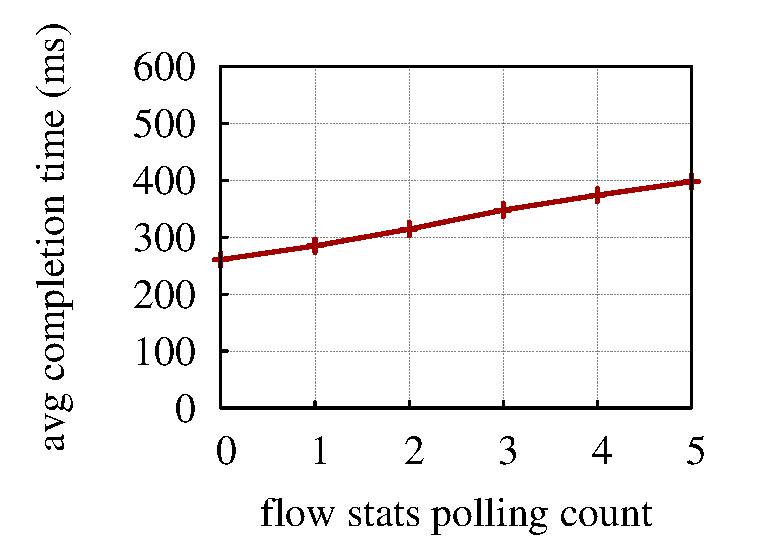
\includegraphics[width=0.25\textwidth]{./figs/bcm_polling_table0_burst100.eps}}
\subfloat[init. table occupancy 500\label{fig:bcm_polling_table500_burst100}]
  {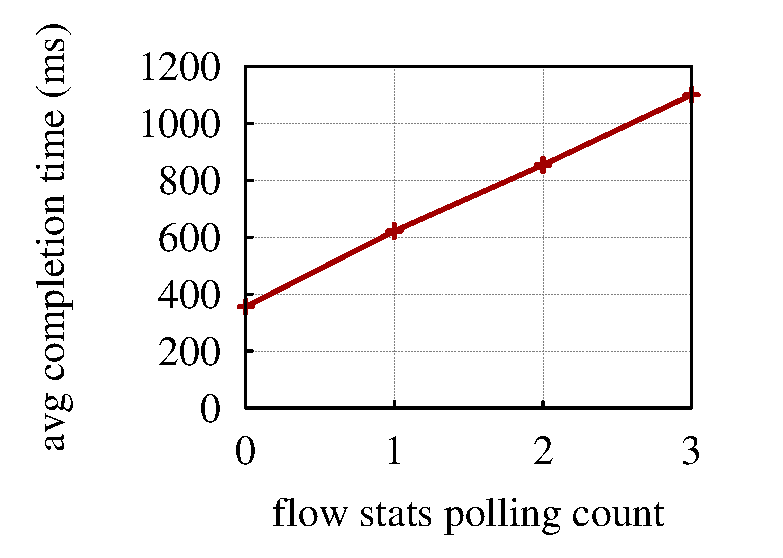
\includegraphics[width=0.25\textwidth]{./figs/bcm_polling_table500_burst100.eps}}\hfill
%\subfloat[controlled-rate mode, rate 50, polling frequency = 1/s\label{fig:bcm_polling_control_50_50_per_polling}]
%  {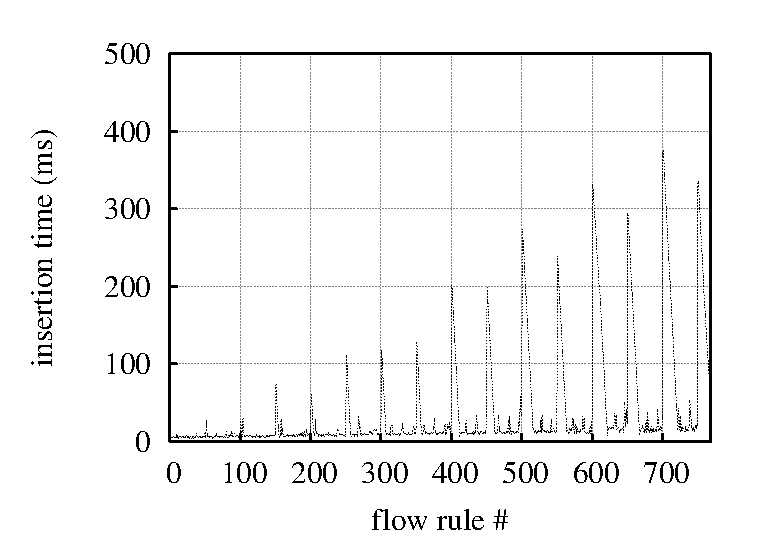
\includegraphics[width=0.3\textwidth]{./figs/bcm_polling_control_50_50_per_polling.eps}}
\topcompactcaption{Impact of polling on {\bf \BroadcomOne}, B=100}
%    ., simple rules (i.e., only specify destination IP)}
%\caption{{\bf Broadcom} per-rule {\bf insert} latency: impact of polling}
\label{fig:polling}
\end{figure}

We previously showed the impact of \flowmod processing on inbound latency
(\secref{s:measure_inbound}). We now study the impact of statistics
polling on outbound latency. 
%In particular,
%To investigate the impact of concurrent switch CPU activities, 
%we instruct the switch to report flow statistics.
%perform flow statistics queries. 
Figure~\ref{fig:polling} shows that concurrent activities, such as polling
statistics, can have a big impact on insertion delay, especially when table
occupancy is high: e.g., with \BroadcomOne, the total time to insert a 
burst of 100 same priority rules into a table with 500 rules is 853ms when 
two polling events occur during the insertion process, compared to
356ms without polling events.
%If we do not poll, the completion
%time of a burst insertion of 100 rules is 280 (xx) ms. If we poll all rules including
%recently installed 10 times during the burst insertion, the
%completion time becomes 490 (xx) ms. 
%\aditya{isn't this polling rate too high?} \aditya{what is the xx supposed to be?}
%$\li{Are we polling existing rule stats? It seems we also poll newly inserted
%  rule stats. What is polling count? }.
\iffalse
\subsection{Overall burst insertion completion time}
With the understanding of per-rule insertion latency, we present burst rule insertion
completion time as this is the metric many applications such as failover depend
on. 

\begin{figure}
\subfloat[insert low priority rules into\newline a table with high priority rules\label{fig:bcm_outbound_two_pri_high_low_burstB}]
  {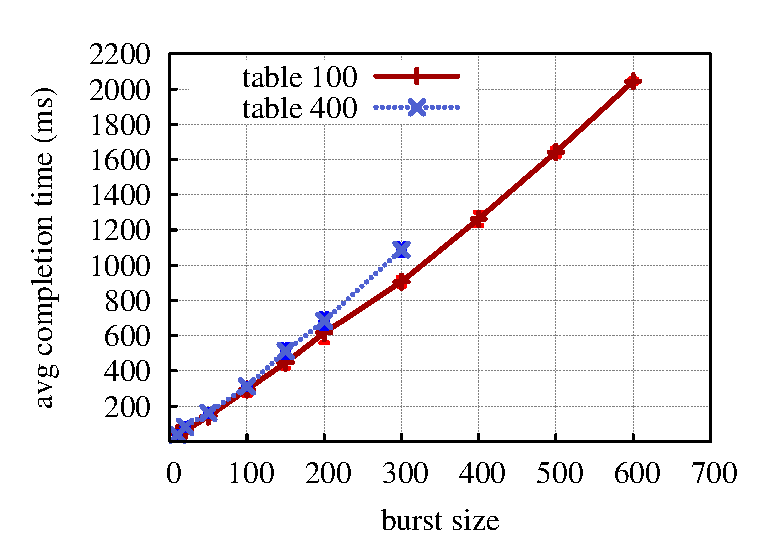
\includegraphics[width=.50\linewidth]{./figs/bcm_two_pri_high_low_burstB.eps}}\hfill
\subfloat[insert high priority rules into a table with low priority rules\label{fig:bcm_outbound_two_pri_low_high_burstB}]
  {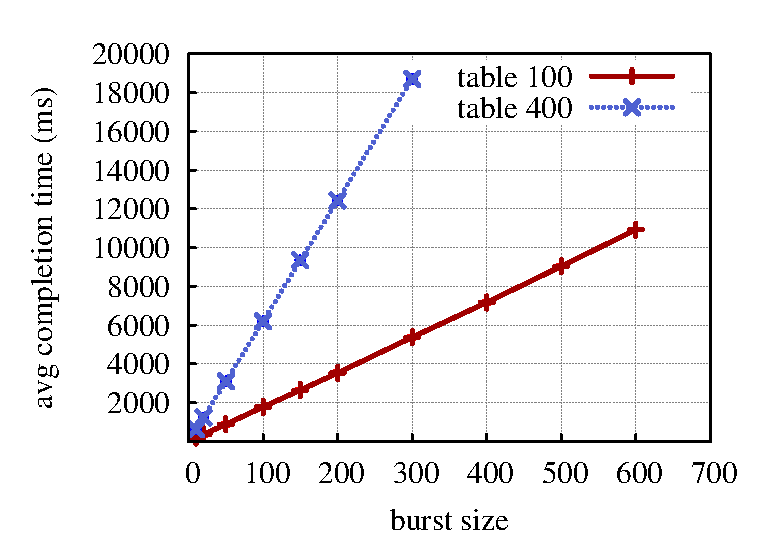
\includegraphics[width=.50\linewidth]{./figs/bcm_two_pri_low_high_burstB.eps}}
\compactcaption{Overall completion time on {\bf \BroadcomOne}.  Initial table
occupancy is S high (low) priority rules; insert a burst of low (high)
priority rules. Averaged over 5 runs. }
\label{fig:burst-completion-time}
\end{figure}
\fi




\iffalse
\begin{figure}[!tb]
\centering
%\subfloat[burst size 100, same priority.\label{fig:intel_burst_100_same_pri}]
%  {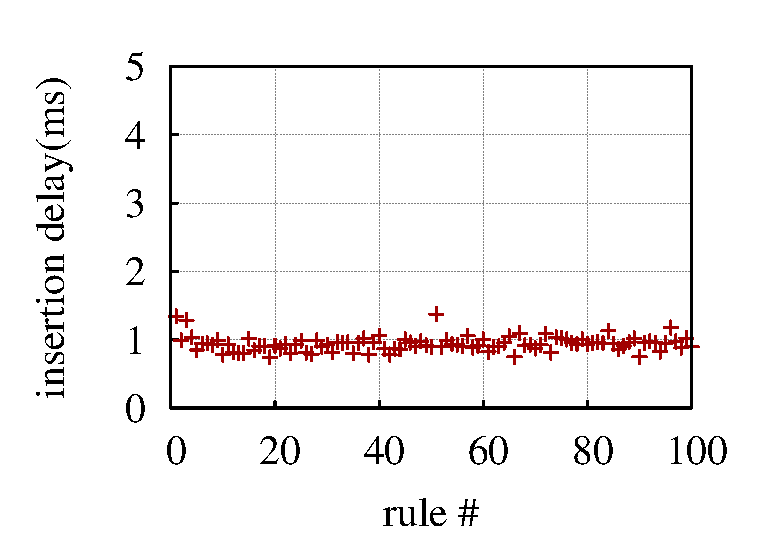
\includegraphics[width=.24\linewidth]{./figs/jan27_intel_same_burst_100.eps}}\hfill
%\subfloat[burst size 200, same priority.\label{fig:intel_burst_200_same_pri}]
%  {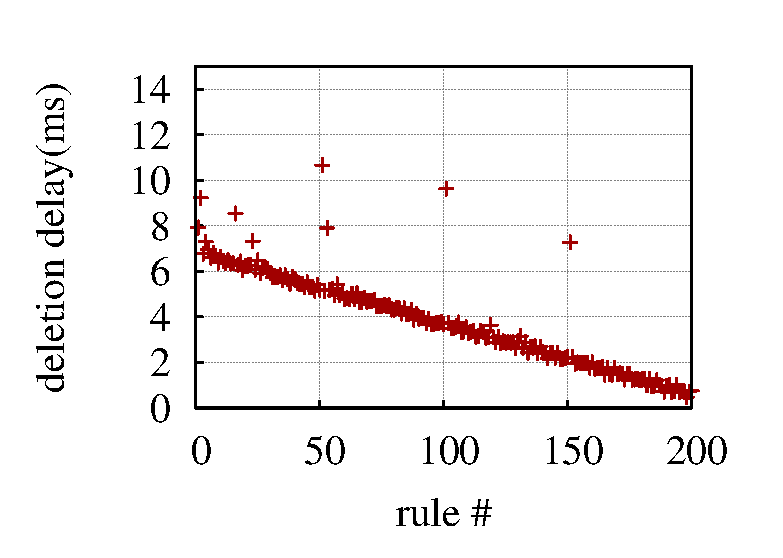
\includegraphics[width=.24\linewidth]{./figs/jan27_intel_same_burst_200.eps}}\hfill
%\subfloat[burst size 800 of low priority, table has 3200 high priority rules\label{fig:intel_burst_200_same_pri}]
%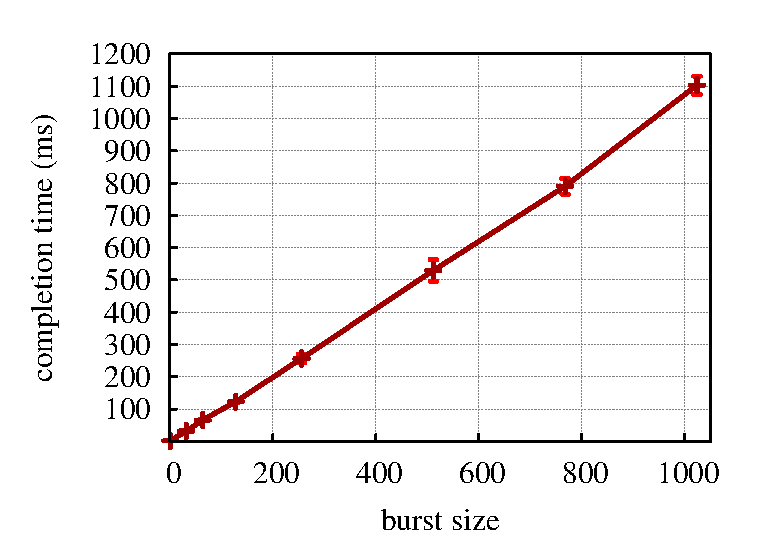
\epsfig{file=./figs/Intel_burst_effect_same.eps,width=0.5\textwidth}
%  {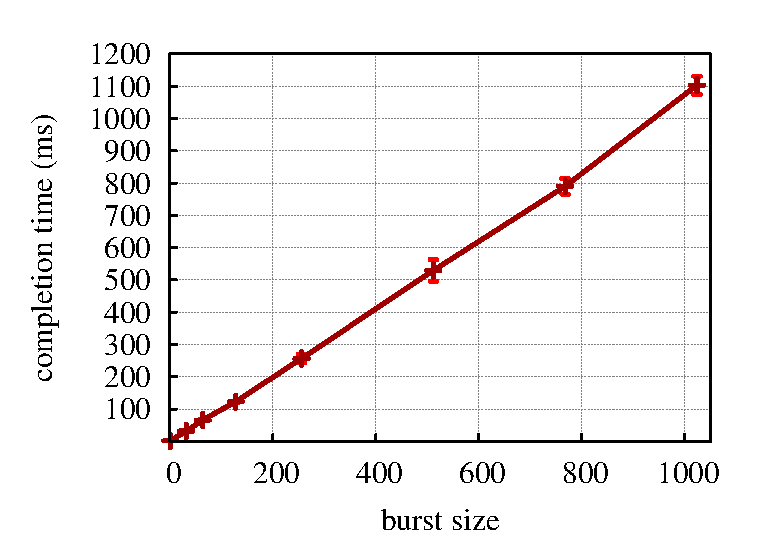
\includegraphics[width=.5\linewidth]{./figs/jan27_intel_burst_effect_same.eps}}\hfill %jan27_intel_decr_burst_100.eps
%   {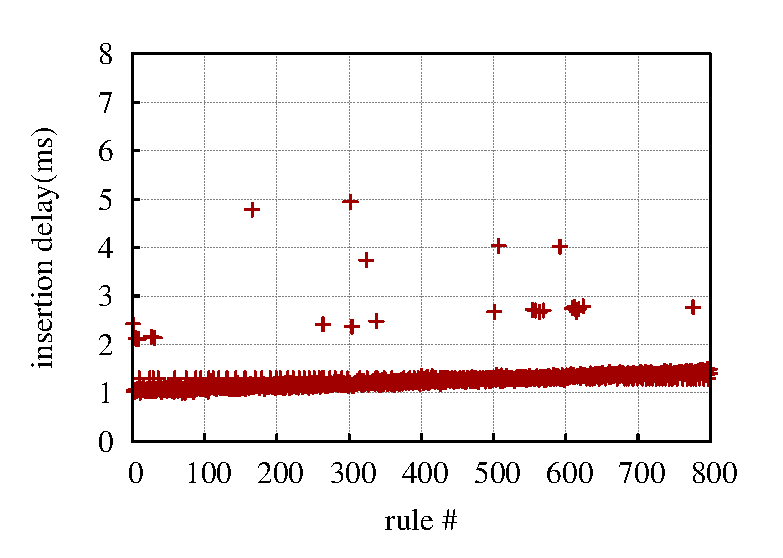
\includegraphics[width=.5\linewidth]{./figs/jan27_intel_3200H_800L_L_to_H_delta.eps}} \hfill
\subfloat[decreasing priority\label{fig:intel_burst_100_incr_pri_1}]
  {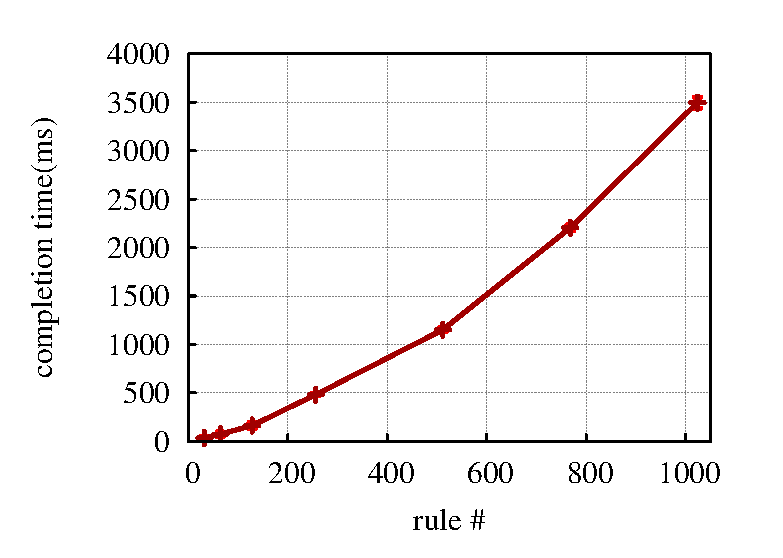
\includegraphics[width=.7\linewidth]{./figs/jan27_intel_decr_burst_size_effect.eps}}\hfill %jan27_intel_decr_burst_100.eps
%\subfloat[burst size 200, decreasing priority.\label{fig:intel_burst_200_incr_pri}]
%  {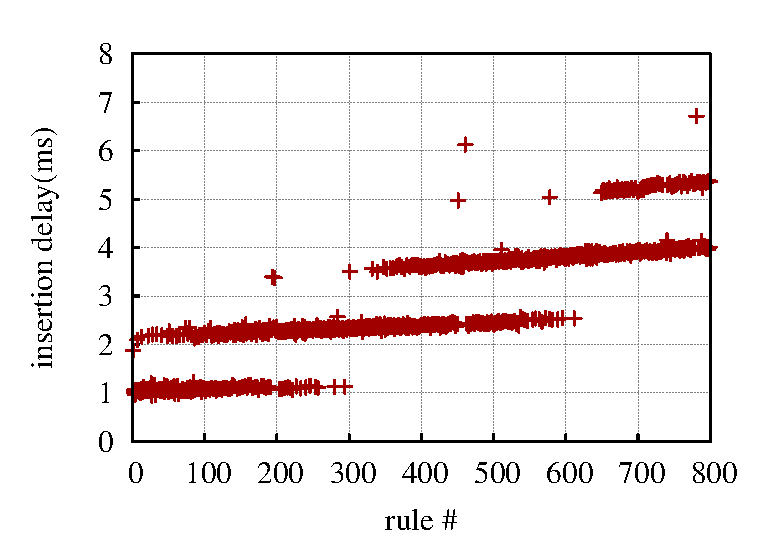
\includegraphics[width=.5\linewidth]{figs/jan27_intel_3200H_800L_decr.eps}}
%\subfloat[burst size 200, decreasing priority.\label{fig:intel_burst_200_decr_pri}]
%  {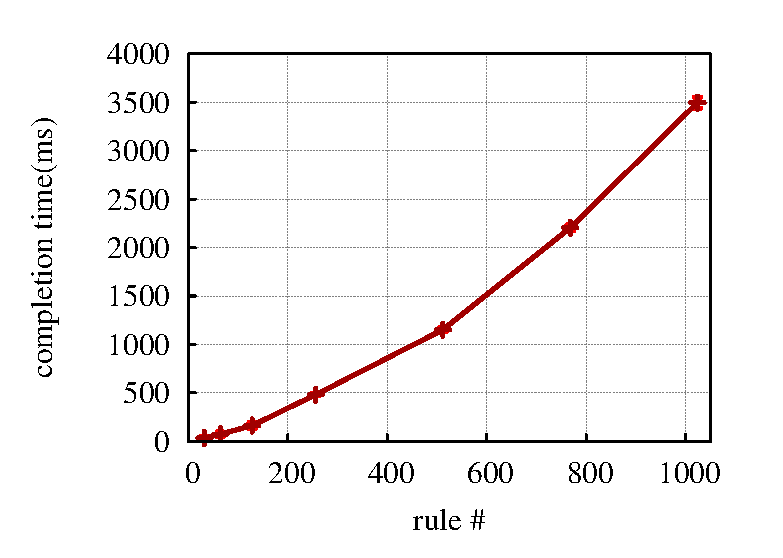
\includegraphics[width=.24\linewidth]{figs/jan27_intel_decr_burst_size_effect.eps}
\caption{{\bf Intel} overall completion time} 
\label{fig:priority-intel-insert-more-results}
\end{figure}
\fi
%\aditya{Is figure 14a correct? It says same priority}
\iffalse
We conduct two experiments. With $S$ rules in the table, we insert a burst of $B$ rules. 
For the first experiment, $S$ has high priority and we insert the burst with low priority. 
For the second experiment, if it is Broadcom (\BroadcomOne or \BroadcomThree), $S$ has low priority and we insert rules with high priority; 
if it is Intel, $S$ has high priority and we insert rules in {\em decreasing} priority.

For Broadcom, based on our hypothesis, as long as the same number of
rules get displaced, the completion time should be the same. Indeed,
 from \figref{fig:bcm_outbound_two_pri_high_low_burstB} (for \BroadcomOne), we see that even with
400 high priority rules in the table, the insertion delay for the
first experiment is no different from the setting when there is only
100 high priority rules in the table. In
\figref{fig:bcm_outbound_two_pri_low_high_burstB}, since newly inserted high
priority rules will displace 400 low priority rules in the table, the
completion time will be about three times higher than $S=100$.
 % If we
% insert in increasing priority, because each rule displaces different
% number of rules (rule $i$ displaces $i-1$ previous inserted rules),
% the total rule displacement is quadratic. Thus, the completion time
% will be quadratic with respect to burst sizes in this case (not
% shown).
%We clearly see this effect in
%Figure~\ref{fig:burst-completion-time-inc}.   
%\li{TODO: Do we need corresponding  results from Intel?} 


%\aditya{the rest does not make full sense. what is ``the first experiment''}

For Intel, % if $S$ has low priority and we insert rules with high priority, then
% it is the same as the first experiment.
we also run the same two experiments as for Broadcom. The results are similar to rule
insertion with same priority. This indicates that Intel optimizes for rule priority better
than Broadcom.  When we insert in decreasing
priority, 
%as shown in Figure~\ref{fig:priority-intel-insert-more-results}, 
the completion time is about 3.5 seconds, three times higher than the case of
insertion with same priority.
%the case in
%Figure~\ref{fig:priority-intel-insert-more-results}-a 
%where we insert a burst of
%800 low priority rules in a table with 3200 high priority rules installed.
%These results provide solid foundations for us to design solutions
%to tame latency in the subsequent sections.
\fi



% LocalWords:  init Broadcom openflow IP justs failover
